\begin{titlingpage}

\includegraphics[width=0.3\textwidth]{Figurer/AU}%~\\[1cm]
\begin{center}
~ \\[0.5cm]

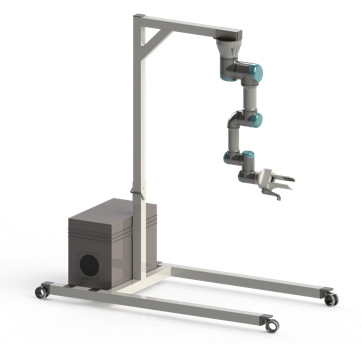
\includegraphics[width=1.0\textwidth]{Figurer/StativMedUR3Render}~\\[1cm]


\textsc{\Large Mini Medicinsk Teknologi Vurdering }\\[0.5cm]

\noindent\makebox[\linewidth]{\rule{\textwidth}{0.4pt}}\\
[0.5cm]{\HUGE Ultralyds Robotarm til scanning af gravide}
\noindent\makebox[\linewidth]{\rule{\textwidth}{0.4pt}}

\end{center}


\vfill

\begin{center}
{\LARGE 2016}
\end{center}

\textbf{Titel}\\
Ultralyds Robotarm til scanning af gravide

\textbf{Udarbejdet af}\\
Anne Bundgaard Hoelgaard\tab 201404492 \newline
Ditte Heebøll Callesen\tab 201408392 \newline
Freja Ramsing Munk\tab 201406736 \newline
Ida Mark Skovbjerg\tab 201404669 \newline	
Mette Østergård Knudsen\tab 201404501 \newline 
Nina Brkovic\tab 201406458 

4. semesterprojekt på sundhedsteknologi, Aarhus Universitet Ingeniørhøjskolen

\textbf{Vejledere} \newline
Lektor Lene Häuser Petersen, \\
Adjunkt Samuel Alberg Thrysøe

\textbf{I samarbejde med}\\
Robotic Ultrasound\\
CEO Søren Pallesen
\\

Afleveringsdato: 30. maj 2016

\end{titlingpage}